%% OTO Open — Original Research submission
%% Double-blind: author information removed from manuscript
\documentclass[12pt,a4paper]{article}

\usepackage{amsmath,amssymb}
\usepackage{graphicx}
\usepackage{booktabs}
\usepackage{multirow}
\usepackage{microtype}
\usepackage[T1]{fontenc}
\usepackage[utf8]{inputenc}
\usepackage[margin=2.5cm]{geometry}
\usepackage{setspace}
\usepackage{lineno}
\usepackage{caption}
\usepackage[superscript,nomove]{cite}   % AMA-style superscript numbered citations
\usepackage[colorlinks=true,linkcolor=blue,citecolor=blue,urlcolor=blue]{hyperref}

\doublespacing
\linenumbers

\begin{document}

% ─────────────────────────────────────────────────────────────────────────────
\begin{center}
{\large\textbf{Predicting Speech-in-Noise Performance Beyond the Pure-Tone
Audiogram: A Machine Learning Benchmark on the Oldenburg Hearing Health
Record}}
\end{center}

\medskip
\noindent\textbf{Running head:} ML Benchmark for Speech-in-Noise Prediction

\medskip
\noindent\textit{[Author information omitted for blinded review]}

% ─────────────────────────────────────────────────────────────────────────────
\section*{Abstract}

\noindent\textbf{Objective.} To benchmark machine learning (ML) models for
predicting speech-in-noise (SIN) performance from progressively richer
audiological feature sets, and to test whether age adds discriminative power
beyond the pure-tone audiogram in an independent population-based sample.

\noindent\textbf{Study Design.} Cross-sectional computational benchmark with
10-fold cross-validation.

\noindent\textbf{Setting.} Single-center audiological clinic (Hörzentrum
Oldenburg, Germany); partial construct validation in the US National Health
and Nutrition Examination Survey (NHANES) 2017--2018.

\noindent\textbf{Methods.} Five feature blocks spanning 1--41 features
(pure-tone audiogram, adaptive loudness scaling, cognition, demographics)
were evaluated in the Oldenburg Hearing Health Record (OHHR; $N=581$ adults,
ages 19--86) using Ridge regression, Random Forest, LightGBM, and a
multilayer perceptron. SHAP analysis identified feature importance. Calibrated
classification of poor SIN performers was assessed by AUROC and Brier score.
Classifiers were applied without retraining to NHANES ($N=859$, ages 70--80)
for partial construct validation against self-reported hearing difficulty.

\noindent\textbf{Results.} A binaural four-frequency pure-tone average (PTA4)
explained 71\% of Digit Triplet Test SIN variance; the full battery achieved
$R^2{=}0.81$ (Random Forest; MAE\,=\,1.23\,dB SNR). Age ranked third in
SHAP importance, above individual audiogram frequencies. Mild hearing loss
(26--40\,dB) benefited most from extended assessment (audiogram-only
$R^2{=}0.09$ vs full battery $R^2{=}0.37$). Poor SIN classification yielded
AUROC\,=\,0.978 (Brier\,=\,0.053). Cross-cohort transfer to NHANES achieved
AUROC\,=\,0.758--0.847 for hearing difficulty; adding age raised AUROC
by $+$0.057.

\noindent\textbf{Conclusion.} The clinical benefit of extended audiological
assessment beyond the audiogram is concentrated in mild hearing loss. Age and
loudness-growth parameters are the most informative non-audiometric predictors,
a finding that partially replicates in an independent general-population cohort.

\medskip
\noindent\textbf{Keywords:} hearing loss, speech in noise, machine learning,
audiology, OHHR, SHAP, calibration, loudness scaling

% ─────────────────────────────────────────────────────────────────────────────
\section{Introduction}

Hearing loss is the third most prevalent chronic condition globally, affecting
an estimated 1.6 billion people, with projections reaching 2.5 billion by
2050.\textsuperscript{1}  Its primary clinical characterisation---the pure-tone
audiogram---measures the softest audible tones across standard frequencies,
yet the audiogram is an incomplete account of real-world hearing function.
A substantial fraction of adults with normal or near-normal audiometric
thresholds report significant difficulty understanding speech in noise
(SIN),\textsuperscript{2} a phenomenon linked to cochlear synaptopathy and
suprathreshold auditory processing deficits.  Conversely, individuals with
similar audiograms can differ markedly in everyday communicative success
owing to differences in cognitive capacity, loudness recruitment, or perceived
hearing quality.\textsuperscript{3}

Predicting SIN performance from audiological measurements has therefore
attracted sustained research interest.  Classical regression studies
established that pure-tone average (PTA) at 0.5--4\,kHz explains roughly
50--70\% of SIN variance in adult cohorts,\textsuperscript{4} and
subsequent work has sought to identify which additional measurements close
the remaining gap.  Cognitive factors---particularly working memory
capacity---have repeatedly been shown to contribute independently of
audiometric thresholds, especially for linguistically demanding sentence
tasks.\textsuperscript{5,6}  Suprathreshold measures of loudness growth from
adaptive categorical loudness scaling (ACALOS) capture outer hair cell
integrity beyond what threshold audiometry detects,\textsuperscript{7} and
several groups have found that loudness parameters add predictive value for
SIN over and above PTA alone.

Recent machine learning (ML) work on large clinical databases has largely
confirmed the PTA--SIN relationship while achieving modest performance
improvements through non-linear modelling.\textsuperscript{8}  However, most
published ML approaches have used narrow feature sets (PTA-only or
demographics plus PTA), have not reported calibrated probabilistic
predictions, have rarely examined severity-stratified utility, and have been
applied to proprietary datasets that preclude direct benchmarking.  The
clinical question of whether extended audiological assessments---beyond the
audiogram---justify their administrative burden for functional hearing
counselling therefore remains open.

The recently published Oldenburg Hearing Health Record
(OHHR)\textsuperscript{9} offers a unique opportunity to address these gaps.
OHHR is an open, CC~BY~4.0 dataset of 581 adults (aged 18--86) containing
air-conduction audiograms, adaptive categorical loudness scaling, digit-triplet
and Göttingen sentence SIN tests, cognitive assessments (DemTect, WortSchatz),
socio-economic indicators, and self-report questionnaires.  Its multimodal
design makes it ideal for disentangling audiometric, auditory-processing,
cognitive, and demographic contributions to functional hearing in a
reproducible benchmark setting.

Our contributions are: (i) the first systematic ML benchmark on OHHR,
comparing five feature blocks spanning 1--41 features and four model
families; (ii) a SHAP-based decomposition of the most informative features
beyond the pure-tone audiogram; (iii) severity-stratified analysis showing
that the clinical benefit of extended assessment is concentrated in mild
hearing loss; (iv) calibrated probabilistic risk predictions for clinical
screening; (v) a neural MLP baseline confirming that tree-ensemble
performance is not capacity-limited on this dataset; and (vi) partial
cross-cohort construct validation on NHANES showing that age improves
audiometric hearing difficulty prediction in an independent general-population
sample.  All code and feature engineering scripts are released openly
[\textit{URL redacted for review}].

% ─────────────────────────────────────────────────────────────────────────────
\section{Materials and Methods}

\subsection{Ethics}

This study analyses pre-existing, publicly available, de-identified datasets
(OHHR, released under CC~BY~4.0, and NHANES, released by the CDC).  No
additional institutional review board approval was required.

\subsection{Dataset}

The Oldenburg Hearing Health Record (OHHR, version~2.0, Zenodo record
16919812\textsuperscript{9}) contains data from 581 adults (255~female,
326~male; age $M{=}67.5{\pm}12.0$\,years, range 19--86) collected between
2013 and 2015 at the Hörzentrum Oldenburg, Germany.  The cohort spans the
full range of clinically relevant hearing loss (better-ear PTA4:
$M{=}31.3{\pm}17.2$\,dB~HL), with 39\% having near-normal thresholds
($\leq$25\,dB) and 31\% having moderate-to-severe loss ($>$40\,dB).
Participant characteristics are summarised in Supplementary Table~S1.
All participants gave written informed consent; data are anonymised and
released under CC~BY~4.0.

\subsection{Feature Extraction}

We constructed 41 features organised into five progressively richer
\textit{feature blocks}:

\textbf{Block~A} (1~feature): binaural four-frequency pure-tone average
(PTA4 mean: mean of left- and right-ear PTA4, where PTA4\,=\,mean of 0.5,
1, 2, and 4\,kHz air-conduction thresholds).

\textbf{Block~B} (14~features): full air-conduction hearing threshold level
(HTL) audiogram at seven frequencies (250--4000\,Hz) per ear.

\textbf{Block~C} (23~features): Block~B plus nine loudness-scaling parameters
from ACALOS---the Brand \& Hohmann (2002) loudness growth function parameters
$m_\text{low}$, $m_\text{high}$, and $m_\text{cut}$ per ear,\textsuperscript{7}
plus mean UCL per ear and inter-ear MCL asymmetry.

\textbf{Block~D} (25~features): Block~C plus DemTect total score (cognitive
screening, 0--18) and WortSchatz verbal intelligence score.

\textbf{Block~E} (41~features): Block~D plus age, sex, education, net income,
hearing aid supply status, hearing loss history flags, and derived audiogram
summaries (better-ear, worse-ear, binaural-mean, and inter-ear-asymmetry
PTA4; high-frequency slope per ear).

Missing values (maximum 3.8\% per feature) were imputed with the
training-fold median; continuous features were standardised for Ridge
regression and the MLP.

\subsection{Cross-Cohort Validation Data}
\label{sec:nhanes}

For partial external validation we used the NHANES 2017--2018 audiometry
module (AUX\_J), hearing questionnaire (AUQ\_J), and demographics
(DEMO\_J).\textsuperscript{10}  NHANES audiometric testing in that cycle was
restricted to adults aged 70--80~years.  After requiring valid pure-tone
thresholds at 0.5, 1, 2, and 4\,kHz bilaterally, the analysis sample
comprised $N{=}859$ participants.  Shared features were: bilateral PTA4
summaries (better, worse, mean, asymmetry), age, and sex.  The primary
validation outcome was AUQ054 (\textit{``How good is your hearing?''},
6-point scale: 1\,=\,excellent, 2\,=\,good, 3\,=\,a little trouble,
4\,=\,moderate trouble, 5\,=\,a lot of trouble, 6\,=\,deaf), dichotomised
as $\geq$3 (any hearing trouble; positive rate 48.8\%).  A secondary outcome
was AUQ101 (\textit{``Difficulty hearing in noise?''}, 5-point scale coded
1\,=\,always \ldots 5\,=\,never), dichotomised as $\leq$2 (always or usually;
positive rate 26.7\%).  Both outcomes are self-report proxies; the analysis
constitutes partial construct validation rather than replication of the OHHR
speech-in-noise endpoint.  Classifiers trained on OHHR were applied without
retraining to the NHANES sample.

\subsection{Prediction Targets}

\textbf{Primary (regression):} Digit Triplet Test (DTT) speech-reception
threshold (SRT, dB~SNR), measured binaurally in free field at 65\,dB~SPL
noise ($M{=}-4.6$\,dB, $SD{=}4.2$\,dB).  Lower SRT indicates better
performance.

\textbf{Secondary (regression):} Göttingen Sentence Test (GST) SRT
($M{=}-1.5$, $SD{=}3.1$\,dB).

\textbf{Classification:} \textit{Poor SIN} defined as DTT
SRT\,${>}{-2}$\,dB~SNR (21.0\% prevalence, $n{=}122$).  This threshold lies
approximately 2.6\,dB above the cohort mean, near the 80th percentile of the
distribution, and demarcates a range where digit-triplet intelligibility
reliably deteriorates in real-world conditions.  The cut-off was selected
\emph{a priori} based on the score distribution without post-hoc optimisation.

\subsection{Models and Evaluation}

Four model families were evaluated for regression: \textbf{Ridge regression}
($\alpha{=}1$); \textbf{Random Forest} (RF; 200~trees, $\sqrt{p}$ features,
min.~leaf~5); \textbf{LightGBM} (500~estimators, learning rate~0.05,
31~leaves, $L_2{=}1.0$); and a \textbf{multilayer perceptron} (MLP;
256/128/64~units, batch normalisation, dropout~0.25, Adam, early
stopping).  For classification, \textbf{logistic regression} (LR) was
additionally evaluated.

Regression performance was quantified as $R^2$ and MAE under 10-fold
cross-validation (CV).  Bootstrap 95\% confidence intervals (2000~resamples,
concatenated out-of-fold predictions) were computed for each model's Block~E
$R^2$.  Pairwise comparisons used the Wilcoxon signed-rank test on per-fold
$R^2$ values (two-sided; $\alpha{=}0.05$).  Classification performance was
evaluated via AUROC, AUPRC, and Brier score under 10-fold stratified CV.

SHAP values\textsuperscript{11} were computed for the LightGBM model trained
on Block~E features.  Stability across the 10~CV folds was quantified by the
coefficient of variation of per-fold mean absolute SHAP values.  A
severity subgroup analysis stratified participants by better-ear PTA4
($\leq$25, 26--40, 41--60, $>$60\,dB~HL) and computed within-stratum 5-fold
Ridge CV $R^2$ for Block~A and Block~E.  A minimal-predictor analysis added
features one at a time in SHAP-ranked order, tracking 10-fold LightGBM CV
$R^2$.

% ─────────────────────────────────────────────────────────────────────────────
\section{Results}

\subsection{DTT SRT Regression Benchmark}

Table~\ref{tab:benchmark} and Figure~\ref{fig:benchmark} summarise regression
performance.  The binaural PTA4-mean baseline (Block~A) already explains
70.8--71.9\% of DTT SRT variance across all models.  Extending to the full
audiogram (Block~B) yields a clear gain for ensemble methods (RF:
$R^2{=}0.790$, LightGBM: $R^2{=}0.732$) but not for Ridge ($R^2{=}0.693$),
suggesting non-linear frequency interactions.  Adding loudness scaling
(Block~C) provides the largest incremental LightGBM gain ($\Delta
R^2{=}0.029$, from 0.732 to 0.761; Wilcoxon $p{=}0.037$), and bootstrap 95\%
CIs for Blocks~B and C partially overlap ($[0.678,\,0.784]$ and
$[0.705,\,0.805]$), indicating a consistent but moderate improvement.
Cognitive measures (Block~D) add only marginally ($\Delta R^2{<}0.002$).  The
full battery (Block~E) achieves the best overall performance:
\textbf{RF: $R^2{=}0.805$, MAE\,=\,1.23\,dB~SNR}; LightGBM Block~E:
$R^2{=}0.772$ (95\%~CI: $[0.728,\,0.811]$; Wilcoxon vs Block~A, $p{=}0.049$).

The GST SRT (sentence test) shows lower overall predictability
($R^2{=}0.57$--$0.67$; best: RF Block~E, $R^2{=}0.672$), consistent with
sentences engaging cognitive processing beyond pure-tone
sensitivity.\textsuperscript{5}

\begin{table}[htbp]
\caption{\textbf{Ten-fold CV regression performance (DTT SRT).}
$R^2$ and MAE (dB SNR) for all model\,$\times$\,feature-block combinations.
Bold indicates the best $R^2$ overall.  95\% CIs are bootstrap intervals
(2000 resamples) on concatenated out-of-fold predictions.}
\label{tab:benchmark}
\centering\small
\begin{tabular}{llccc}
\toprule
Feature block & Model & $R^2$ & MAE (dB) & 95\% CI ($R^2$) \\
\midrule
\multirow{3}{*}{A: PTA4 mean (1 feat.)}
  & Ridge     & 0.708 & 1.602 & -- \\
  & RF        & 0.719 & 1.482 & -- \\
  & LightGBM  & 0.715 & 1.507 & [0.645, 0.766] \\
\midrule
\multirow{3}{*}{B: Full PTA (14 feat.)}
  & Ridge     & 0.693 & 1.651 & -- \\
  & RF        & 0.790 & 1.274 & -- \\
  & LightGBM  & 0.732 & 1.436 & [0.678, 0.784] \\
\midrule
\multirow{3}{*}{C: +Loudness (23 feat.)}
  & Ridge     & 0.695 & 1.652 & -- \\
  & RF        & 0.797 & 1.255 & -- \\
  & LightGBM  & 0.761 & 1.374 & [0.705, 0.805] \\
\midrule
\multirow{3}{*}{D: +Cognition (25 feat.)}
  & Ridge     & 0.693 & 1.654 & -- \\
  & RF        & 0.796 & 1.254 & -- \\
  & LightGBM  & 0.762 & 1.365 & [0.710, 0.808] \\
\midrule
\multirow{3}{*}{E: Full battery (41 feat.)}
  & Ridge     & 0.730 & 1.566 & [0.687, 0.761] \\
  & RF        & \textbf{0.805} & \textbf{1.227} & [0.756, 0.836] \\
  & LightGBM  & 0.772 & 1.333 & [0.728, 0.811] \\
\bottomrule
\end{tabular}
\end{table}

\subsection{Feature Importance and Stability}

Figure~\ref{fig:shap} shows mean absolute SHAP values for the LightGBM
Block~E model.  The better-ear PTA4 summary dominates
($\overline{|\phi|}{=}1.82$).  The 2\,kHz right-ear threshold ranks second
($\overline{|\phi|}{=}0.32$), consistent with the importance of the
high-frequency audiogram slope.\textsuperscript{12}  \textbf{Age ranks third}
($\overline{|\phi|}{=}0.29$), overtaking all individual audiogram frequencies,
underscoring age-related suprathreshold processing
changes.\textsuperscript{13}  The loudness-scaling slope $m_\text{low}$ (left
ear) ranks 4th ($\overline{|\phi|}{=}0.26$), the first non-audiometric,
non-demographic feature.  Cognitive measures (DemTect, verbal intelligence)
rank below audiogram features.  Figure~\ref{fig:comparison}b shows SHAP
stability across the 10~CV folds; top features have coefficient-of-variation
$<$0.15.

\subsection{Severity-Stratified Analysis}

Figure~\ref{fig:subgroup}a reveals a clinically important severity-dependent
pattern.  For \textbf{mild hearing loss} (26--40\,dB, $n{=}174$),
audiogram-only Ridge regression explains only $R^2{=}0.089$ of DTT variance;
the full battery raises this to $0.368$ ($+$0.28 absolute, a 4$\times$
improvement), reflecting the dominance of suprathreshold variance in this
group.  For \textbf{near-normal thresholds} ($\leq$25\,dB, $n{=}228$),
extended features similarly improve prediction ($R^2$: $0.395\to0.583$).
For \textbf{moderate hearing loss} (41--60\,dB, $n{=}148$), PTA4 alone
achieves $R^2{=}0.310$, but adding the full feature set reduces $R^2$ to
$0.020$---a sharp decline reflecting reduced DTT variance in this severity
stratum and an elevated feature-to-sample ratio in 5-fold CV; this finding
cautions against applying the full battery in moderate-loss subgroups without
larger cohort sizes or stronger regularisation.  The severe-loss group
($>$60\,dB, $n{=}31$) is too small for reliable within-subgroup CV.

\subsection{Classification and Calibration}

Table~\ref{tab:classification} reports classification performance for the
\textit{poor SIN} target.  Both LR (Block~A) and LightGBM (Block~E) achieve
high discrimination (AUROC\,$>$\,0.96).  LightGBM Block~E reaches
\textbf{AUROC\,=\,0.978, AUPRC\,=\,0.938} (95\%~CI for AUROC: [0.966, 0.987]).
Brier scores are low (LR: 0.058; LightGBM: 0.053), and calibration curves
(Figure~\ref{fig:subgroup}b) show close agreement between predicted
probabilities and observed event rates across the cross-validated risk range,
indicating well-calibrated probabilities within this cohort; prospective
external validation would be needed before clinical deployment.

\begin{table}[htbp]
\caption{\textbf{Classification performance (poor SIN: DTT SRT $>{-2}$\,dB).}
AUROC, AUPRC, and Brier score under 10-fold stratified CV.}
\label{tab:classification}
\centering\small
\begin{tabular}{llccc}
\toprule
Block & Model & AUROC & AUPRC & Brier \\
\midrule
A: PTA4 mean  & LR        & 0.965 & 0.881 & 0.058 \\
B: Full PTA   & LR        & 0.966 & 0.895 & --   \\
B: Full PTA   & LightGBM  & 0.955 & 0.893 & --   \\
C: +Loudness  & LightGBM  & 0.968 & 0.914 & --   \\
E: Full batt. & LR        & 0.969 & 0.919 & --   \\
E: Full batt. & LightGBM  & \textbf{0.978} & \textbf{0.938} & \textbf{0.053} \\
\bottomrule
\end{tabular}
\end{table}

\subsection{Minimal Predictor Analysis}

The single best SHAP-ranked feature (PTA4-better alone) achieves $R^2{=}0.765$
in 10-fold LightGBM CV---exceeding the binaural PTA4-mean Block~A baseline
($R^2{=}0.708$--$0.719$) and confirming the SHAP ranking's predictive
validity.  The top-3 features (PTA4-better, 2\,kHz right-ear HTL, age) yield
$R^2{=}0.738$, within 0.034 of the full-battery model ($R^2{=}0.772$), and
the top-7 features ($R^2{=}0.741$) exceed LightGBM Block~B ($R^2{=}0.732$)
at a fraction of the measurement burden.  Performance stabilises near the
full-battery level at approximately 15--20 features ($R^2{=}0.766$--$0.784$).

\subsection{Neural Baseline}

Figure~\ref{fig:comparison}a compares all four model families on Block~E.
The MLP achieves $R^2{=}0.795\pm0.059$ and MAE\,=\,$1.28\pm0.19$\,dB~SNR
under 10-fold CV---not significantly different from RF ($R^2{=}0.805$;
Wilcoxon $p{=}0.625$) or LightGBM ($R^2{=}0.772$; $p{=}0.232$), but
significantly above Ridge ($R^2{=}0.730$; $p{=}0.006$).

\subsection{Cross-Cohort Partial Validation}

Table~\ref{tab:crosscohort} and Figure~\ref{fig:crosscohort} summarise the
NHANES transfer results.  A PTA4-only model trained on OHHR achieves
AUROC\,=\,0.758 for predicting NHANES general hearing difficulty (AUQ054)---above
chance despite the distributional shift between a German clinical cohort and a
US general-population survey.  Adding age (PTA4\,+\,Age) raises the NHANES
AUROC to 0.815 ($\Delta{=}+0.057$), corroborating that age is an informative
predictor beyond threshold sensitivity.  The matched 8-frequency HTL model
achieves AUROC\,=\,0.847.  For the speech-in-noise specific item (AUQ101,
$\leq$2 coded as positive), transfer AUROCs are somewhat lower but still
well above chance (PTA4-only: 0.695; PTA4\,+\,Age: 0.744; matched HTL\,+\,Age:
0.764), consistent with SIN difficulty being a more specific and
harder-to-predict construct than general hearing difficulty.

\begin{table}[htbp]
\caption{\textbf{Cross-cohort transfer: OHHR $\to$ NHANES ($N{=}859$, ages
70--80).}  OHHR AUROC is out-of-fold; NHANES AUROCs evaluate dichotomised
AUQ054 (general hearing difficulty, $\geq$3) and AUQ101 (SIN difficulty,
$\leq$2).}
\label{tab:crosscohort}
\centering\small
\begin{tabular}{lccc}
\toprule
Feature set & OHHR AUROC & NHANES AUQ054 & NHANES AUQ101 \\
            & (OOF)      & (hearing diff.) & (SIN diff.) \\
\midrule
PTA4 only         & 0.943 & 0.758 & 0.695 \\
PTA4 + Age        & 0.968 & 0.815 & 0.744 \\
PTA4 + Age + Sex  & 0.968 & 0.811 & 0.745 \\
Matched HTL + Age & 0.958 & \textbf{0.847} & \textbf{0.764} \\
\bottomrule
\end{tabular}
\end{table}

% ─────────────────────────────────────────────────────────────────────────────
\section{Discussion}

Our benchmark establishes several findings with direct clinical relevance.

\textbf{The audiogram is efficient but not sufficient.}  A single binaural
PTA4 summary explains 71\% of DTT SRT variance, confirming decades of
audiological knowledge,\textsuperscript{4} yet the remaining 29\% carries
clinically meaningful signal---particularly in mild hearing loss, where the
audiogram approaches chance-level prediction of SIN ability.  This is
consistent with the broader literature on suprathreshold auditory processing,
where outer hair cell integrity (reflected in loudness growth) and central
auditory function (correlated with age and cognition) contribute independently
to SIN performance.\textsuperscript{14}

\textbf{Loudness scaling is the most valuable non-audiometric measure.}
ACALOS-derived parameters outrank cognitive scores in SHAP importance (though
age ranks above the first loudness parameter).  The loudness slope
$m_\text{low}$ reflects cochlear amplifier gain, which degrades with outer
hair cell loss and modulates dynamic range adaptation in
noise.\textsuperscript{7}  Clinically, a brief ACALOS procedure added to
routine audiometry should provide meaningful incremental benefit for counselling,
especially in mild-loss patients where the audiogram is least informative.

\textbf{Extended assessment benefit is severity-dependent.}  For mild hearing
loss (26--40\,dB~HL), the audiogram explains only 9\% of SIN variance and
the full battery yields a fourfold improvement ($R^2{=}0.368$).  These are
the patients most likely to be in the grey zone of hearing aid candidacy,
where audiogram-only counselling is least reliable.  For moderate hearing loss
(41--60\,dB), Ridge regression with the full battery drops to $R^2{=}0.020$
from $R^2{=}0.310$ with PTA only, suggesting overfitting in the small stratum
rather than genuine feature utility; this deserves reassessment with a larger
moderate-loss cohort.

\textbf{Neural vs.\ tree-based models.}  The MLP matches RF ($R^2{=}0.795$
vs.\ $0.805$) but does not significantly outperform it (Wilcoxon $p{=}0.625$),
consistent with the tabular learning literature where gradient boosting
typically matches or exceeds neural networks at this dataset
scale.\textsuperscript{15}

\textbf{Cross-cohort generalisability.}  The NHANES transfer results (AUQ054
AUROC 0.76--0.85; AUQ101 AUROC 0.69--0.76) suggest that OHHR-trained models
retain meaningful discriminative power in an independent general-population
sample.  Adding age raises NHANES AUQ054 AUROC by $+0.057$, corroborating
the SHAP-identified importance of age beyond the audiogram in a second cohort.
These results should be interpreted cautiously: both NHANES outcomes are
single self-report items, not standardised administered SIN tests, so the
transfer constitutes partial construct validation rather than direct
replication of the OHHR clinical endpoint.

\textbf{Comparison to prior work.}  Our best result ($R^2{=}0.81$, RF
Block~E) is consistent with the upper range of PTA-based SIN prediction in
the literature ($r^2{\approx}0.50$--$0.70$ for older clinical
populations\textsuperscript{4}).  In contrast to Ng et al.,\textsuperscript{5}
who found cognitive measures substantially improved SIN prediction, we find
only marginal improvement from DemTect and vocabulary scores, possibly because
the DTT digit task is less cognitively demanding than sentence tests.  The
OHHR benchmark also directly extends prior ML work by Gathman et al.,\textsuperscript{8}
which demonstrated ML prediction of objective hearing loss; the present study
additionally provides severity stratification, probability calibration, and
cross-cohort validation that were absent from prior reports.

\textbf{Limitations.}  The OHHR cohort was collected at a single German
centre (2013--2015) with limited ethnic and geographic diversity.  Audiogram
frequencies extend to 4\,kHz only, omitting extended high-frequency thresholds
(6--8\,kHz) linked to cochlear health.\textsuperscript{2}  Hearing aid use
during DTT testing could not be fully controlled.  The NHANES validation is
partial: the sample ($N{=}859$, ages 70--80) is restricted to older adults,
and NHANES audiometry covers only 500--4\,kHz.  Crucially, the NHANES
validation targets (AUQ054 and AUQ101) are single self-report Likert items,
not administered SIN tests; self-report and performance measures tap partly
distinct constructs (perceived handicap vs.\ objective signal detection), so
AUROC values on these items cannot be compared directly to AUROC values on
administered SIN endpoints.  The moderate-loss subgroup showed a sharp Ridge
$R^2$ decline (0.310$\to$0.020) with the full feature set, likely reflecting
overfitting; future work should verify this with a larger cohort and stronger
regularisation.  Finally, with $n{=}10$ folds the Wilcoxon test has limited
power for subtle performance differences.

% ─────────────────────────────────────────────────────────────────────────────
\section{Conclusion}

The benefit of extended audiological assessment beyond the pure-tone audiogram
is concentrated in mild hearing loss (26--40\,dB), where audiogram-alone
prediction is near chance ($R^2{=}0.09$) and a broader battery achieves
$R^2{=}0.37$.  Age and loudness-growth parameters are the most informative
non-audiometric predictors; this finding partially replicates in independent
NHANES data ($N{=}859$, ages 70--80), where adding age to a PTA4-only model
raises cross-cohort AUROC from 0.758 to 0.815.  Calibrated classification of
poor SIN performers achieves AUROC\,=\,0.978 with well-calibrated probability
estimates within this cohort, supporting the clinical utility of probabilistic
audiological risk screening in mild hearing loss---the population where
audiogram-only counselling is least reliable.  All code is released openly
[\textit{URL available upon acceptance}] to facilitate future benchmarking.

% ─────────────────────────────────────────────────────────────────────────────
\section*{Acknowledgments}

We thank the OHHR team at the Hörzentrum Oldenburg and the Hearing4all Cluster
of Excellence for making this dataset publicly available under an open licence.

% ─────────────────────────────────────────────────────────────────────────────
\section*{Author Contributions}

\textit{[Omitted for blinded review.]}

\section*{Competing Interests}

The authors declare no competing interests.

\section*{Data Availability}

The OHHR dataset is publicly available at Zenodo
(DOI:~10.5281/zenodo.16919812) under CC~BY~4.0.  NHANES 2017--2018 data are
publicly available from the CDC (\url{https://wwwn.cdc.gov/nchs/nhanes}).

\section*{Code Availability}

Feature engineering scripts, model training code, per-fold results, and
pre-trained model weights are available at [\textit{URL redacted for review}]
under the MIT licence.

% ─────────────────────────────────────────────────────────────────────────────
\begin{thebibliography}{15}

\bibitem{who2021}
World Health Organization. \textit{World Report on Hearing}. WHO; 2021.

\bibitem{Plack2014}
Plack CJ, Barker A, Prendergast G. Perceptual consequences of ``hidden''
hearing loss. \textit{Trends Hear}. 2014;18:2331216514550621.

\bibitem{Gatehouse2004}
Gatehouse S, Noble W. The speech, spatial and qualities of hearing scale
(SSQ). \textit{Int J Audiol}. 2004;43(2):85-99.

\bibitem{Smoorenburg1992}
Smoorenburg GF. Speech reception in quiet and in noisy conditions by
individuals with noise-induced hearing loss in relation to their tone
audiogram. \textit{J Acoust Soc Am}. 1992;91(1):421-437.

\bibitem{Ng2015}
Ng EHN, Classon E, Larsby B, et al. Dynamic relation between working memory
capacity and speech recognition in noise during the first 6 months of hearing
aid use. \textit{Trends Hear}. 2015;19:2331216515597207.

\bibitem{Lunner2003}
Lunner T. Cognitive function in relation to hearing aid use.
\textit{Int J Audiol}. 2003;42(suppl 1):S49-S58.

\bibitem{Brand2002}
Brand T, Hohmann B. An adaptive procedure for categorical loudness scaling.
\textit{J Acoust Soc Am}. 2002;112(4):1597-1604.

\bibitem{Gathman2023}
Gathman TJ, Choi JS, Vasdev RMS, Schoephoerster JA, Adams ME. Machine
learning prediction of objective hearing loss with demographics, clinical
factors, and subjective hearing status. \textit{Otolaryngol Head Neck Surg}.
2023;169(3):504-513.

\bibitem{OHHR2025}
Kollmeier B, et al. The Oldenburg Hearing Health Record (OHHR).
\textit{Sci Data}. 2025;12:1546.

\bibitem{NHANES2018}
Centers for Disease Control and Prevention. National Health and Nutrition
Examination Survey: Audiometry Data Documentation, AUX\_J 2017--2018.
National Center for Health Statistics; 2020.

\bibitem{Lundberg2017}
Lundberg SM, Lee S-I. A unified approach to interpreting model predictions.
\textit{Adv Neural Inf Process Syst}. 2017;30:4765-4774.

\bibitem{vanRooij1990}
van Rooij JCGM, Plomp R. Auditive and cognitive factors in speech perception
by elderly listeners, II: Multivariate analyses.
\textit{J Acoust Soc Am}. 1990;88(6):2611-2624.

\bibitem{Wingfield2005}
Wingfield A, Tun PA, McCoy SL. Hearing loss in older adulthood: what it is
and how it interacts with cognitive performance.
\textit{Curr Dir Psychol Sci}. 2005;14(3):144-148.

\bibitem{Moore2001}
Moore BCJ. Dead regions in the cochlea: diagnosis, perceptual consequences,
and implications for the fitting of hearing aids.
\textit{Trends Amplif}. 2001;5(1):1-34.

\bibitem{Gorishniy2021}
Gorishniy Y, Rubachev I, Khrulkov V, Babenko A. Revisiting deep learning
models for tabular data. \textit{Adv Neural Inf Process Syst}.
2021;34:18363-18374.

\end{thebibliography}

% ─────────────────────────────────────────────────────────────────────────────
\clearpage

%% FIGURES
\begin{figure}[htbp]
  \centering
  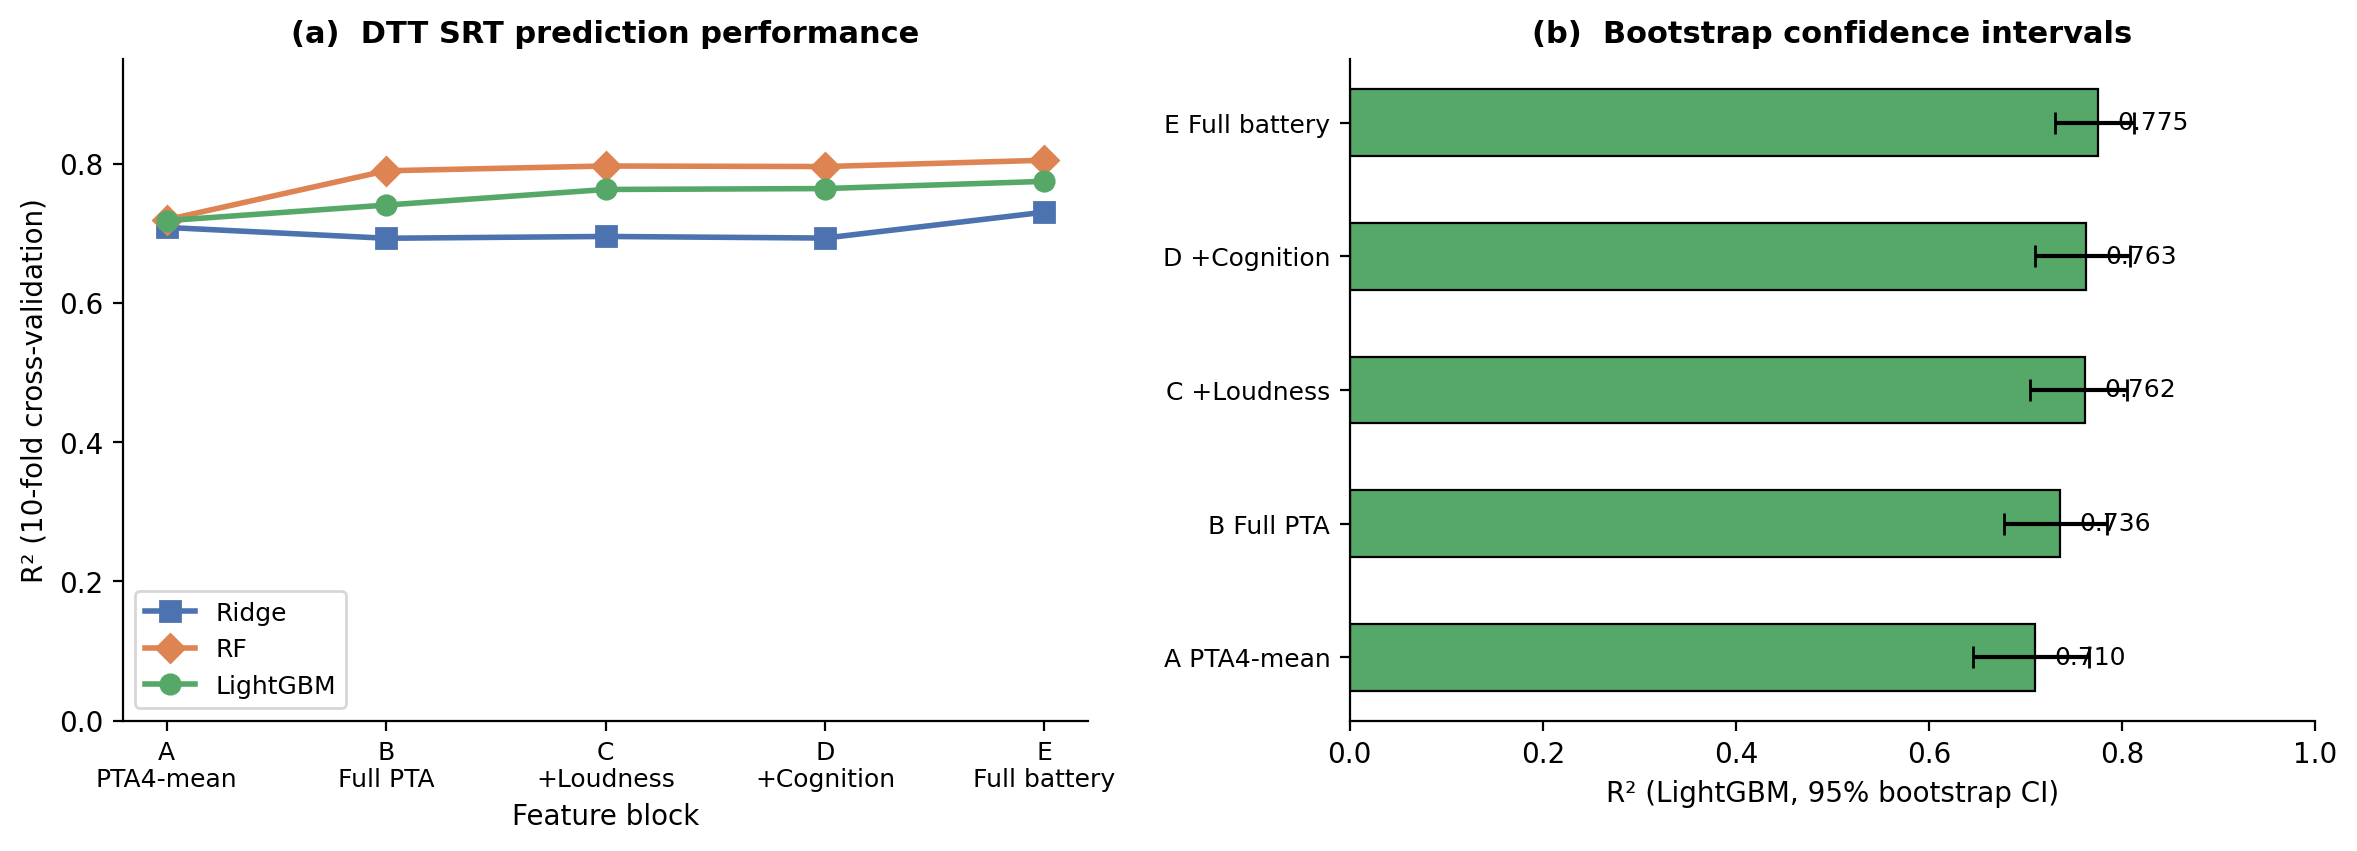
\includegraphics[width=\textwidth]{fig2_benchmark.png}
  \caption{\textbf{DTT SRT prediction performance across feature blocks and
  models.}  \textbf{(A)}~Ten-fold CV $R^2$ for all model\,$\times$\,block
  combinations.  Ensemble methods benefit from extended blocks; Ridge
  performance is more stable.  \textbf{(B)}~Bootstrap 95\% confidence
  intervals for LightGBM $R^2$ by block; intervals partially overlap between
  Blocks~B and C, indicating a consistent but moderate benefit from loudness
  features.}
  \label{fig:benchmark}
\end{figure}

\begin{figure}[htbp]
  \centering
  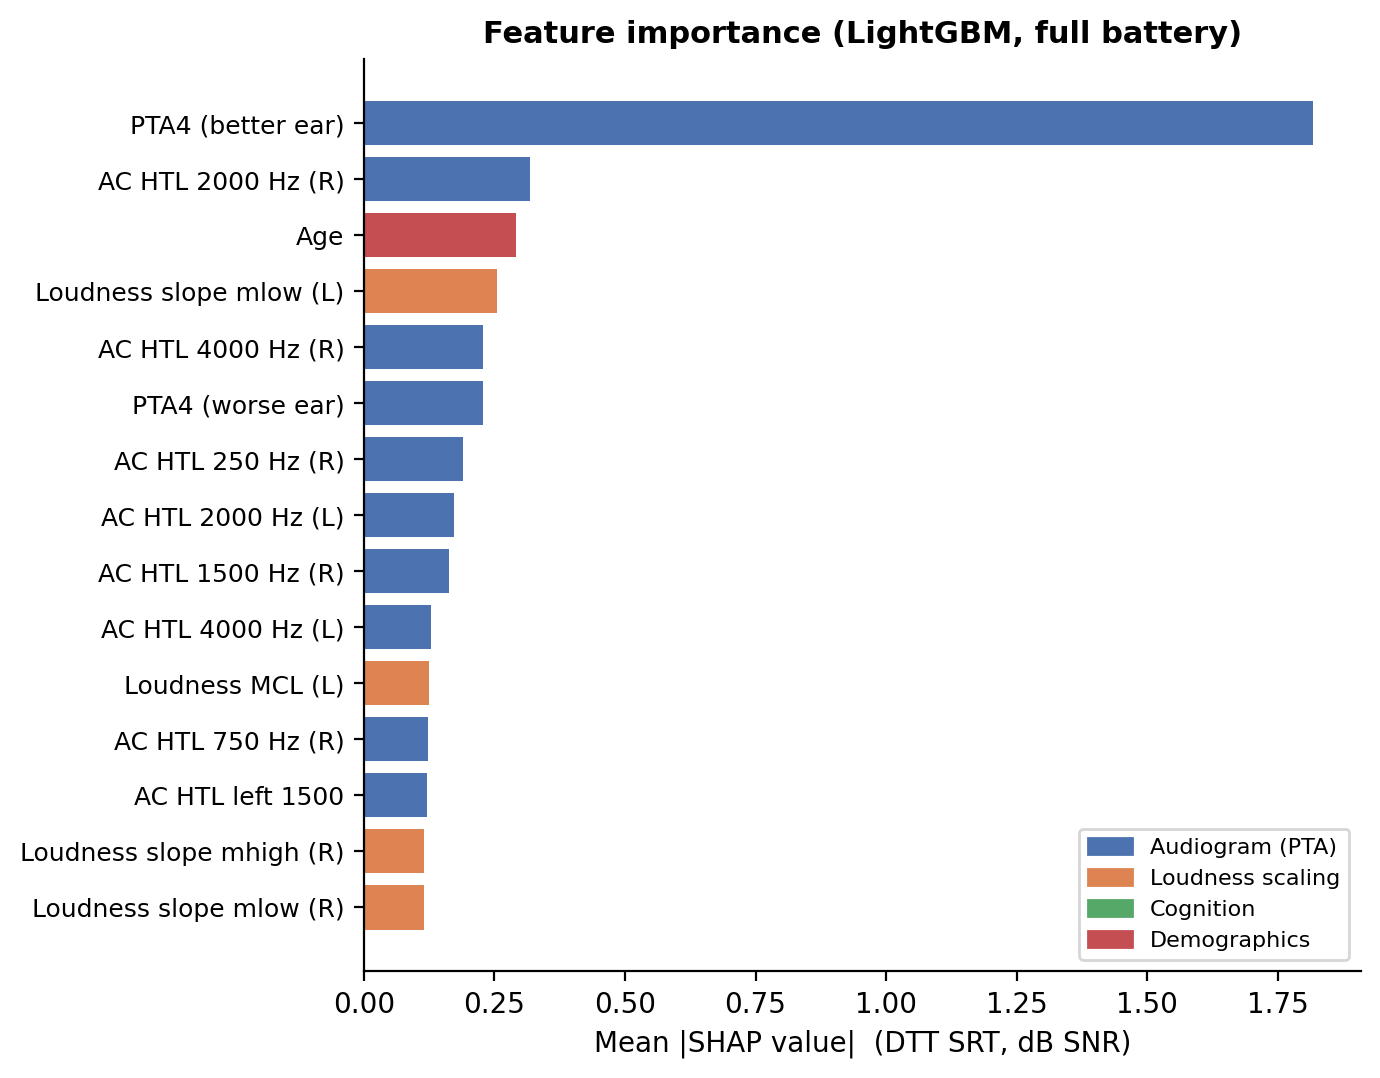
\includegraphics[width=0.75\textwidth]{fig3_shap.png}
  \caption{\textbf{SHAP feature importance (LightGBM, Block~E, top 15
  features).}  Colours indicate feature type: blue\,=\,audiogram, orange\,=\,loudness
  scaling, green\,=\,cognition, red\,=\,demographics.  Beyond the dominant
  PTA4 summary, age (rank 3) and loudness growth slope $m_\text{low}$
  (rank 4) are the most informative predictors.}
  \label{fig:shap}
\end{figure}

\begin{figure}[htbp]
  \centering
  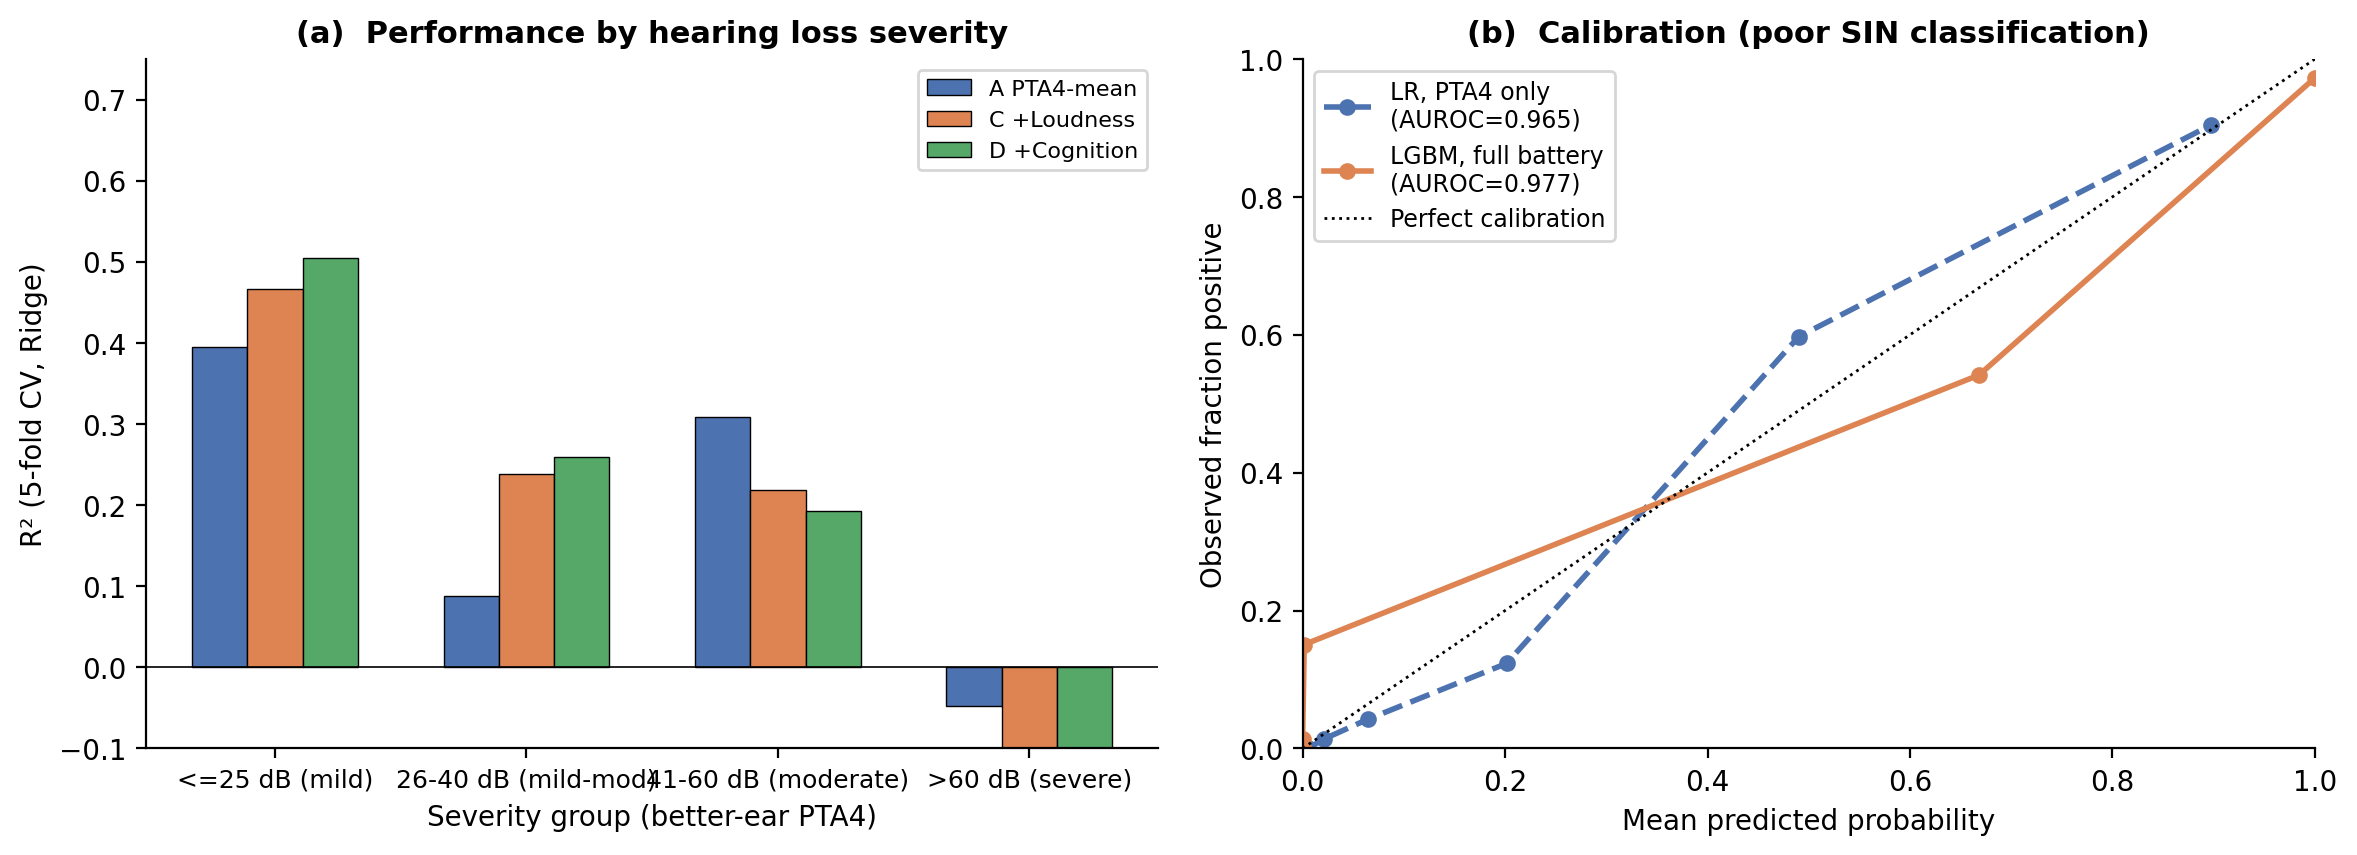
\includegraphics[width=\textwidth]{fig4_subgroup_calibration.png}
  \caption{\textbf{Severity-stratified analysis and calibration.}
  \textbf{(A)}~Within-stratum 5-fold Ridge $R^2$ for Block~A (PTA4 only) and
  Block~E (full battery).  The benefit of extended assessment is concentrated
  in mild hearing loss (26--40\,dB), where PTA4 alone explains only 9\% of
  SIN variance.
  \textbf{(B)}~Calibration curves for LR (Block~A) and LightGBM (Block~E)
  predicting poor SIN performers; both models show close agreement with the
  diagonal across the cross-validated risk range.}
  \label{fig:subgroup}
\end{figure}

\begin{figure}[htbp]
  \centering
  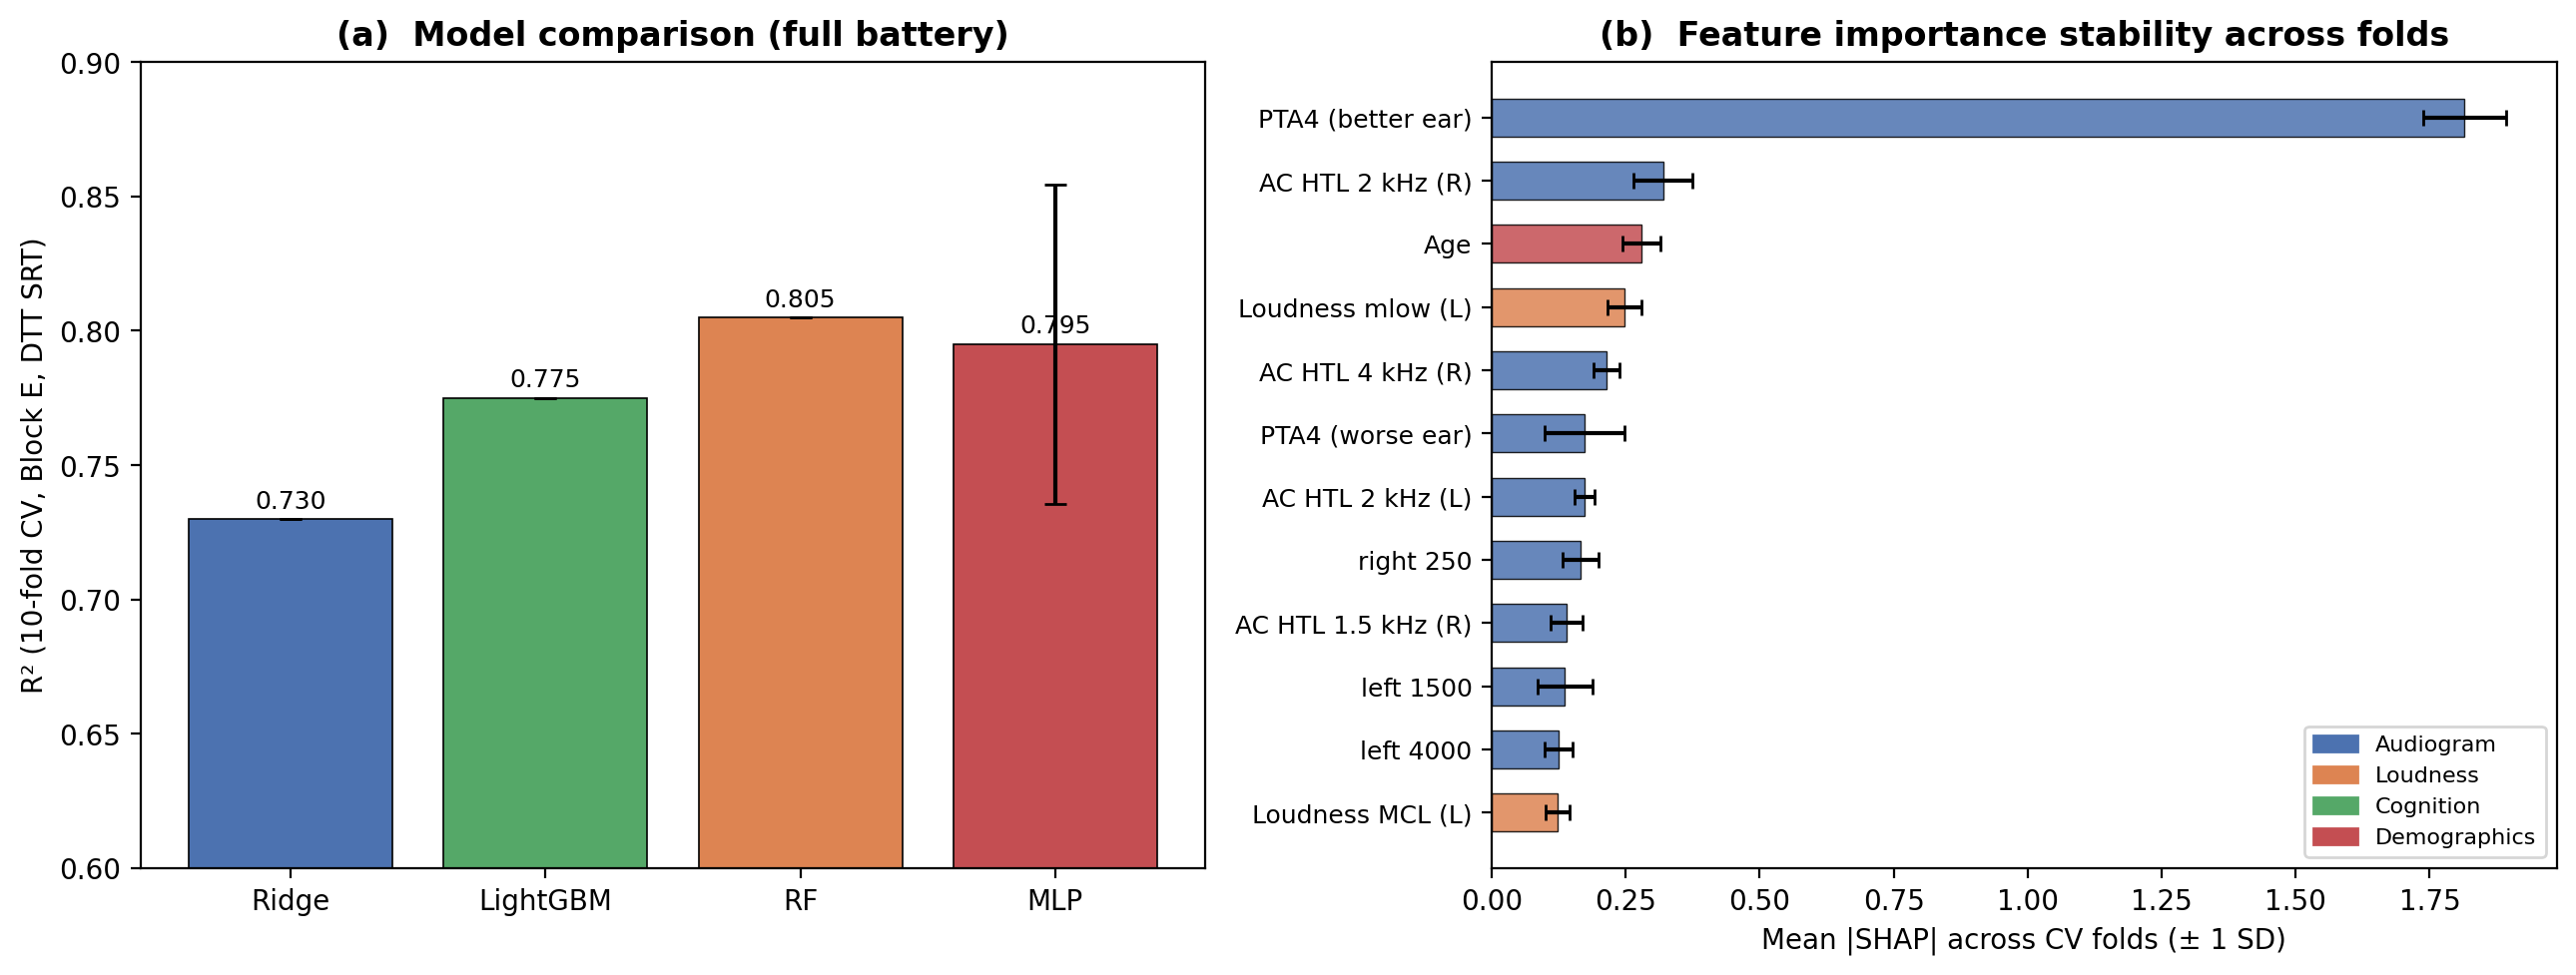
\includegraphics[width=\textwidth]{fig6_model_comparison_stability.png}
  \caption{\textbf{Model comparison and SHAP stability.}
  \textbf{(A)}~Block~E $R^2$ for Ridge, LightGBM, RF, and MLP.
  \textbf{(B)}~Mean absolute SHAP values with fold-level SD ($\pm$1~SD
  error bars); top features have coefficient-of-variation\,$<$\,0.15,
  confirming ranking stability.}
  \label{fig:comparison}
\end{figure}

\begin{figure}[htbp]
  \centering
  
\includegraphics[width=\textwidth]{fig5_crosscohort.png}
  \caption{\textbf{Cross-cohort validation: OHHR $\to$ NHANES.}
  \textbf{(A)}~AUROC for predicting NHANES self-reported hearing difficulty
  (AUQ054) by feature set; adding age to PTA4 raises AUROC from 0.758 to
  0.815.
  \textbf{(B)}~Distribution of predicted P(poor SIN) by NHANES AUQ054
  category (1\,=\,excellent, 5\,=\,a lot of trouble, 6\,=\,deaf); predicted
  risk increases monotonically with hearing difficulty category.
  \textbf{(C)}~OOF calibration curves on OHHR for PTA4-only and PTA4\,+\,Age
  classifiers.}
  \label{fig:crosscohort}
\end{figure}

%% SUPPLEMENTARY
\clearpage
\section*{Supplementary Information}

\setcounter{table}{0}
\renewcommand{\thetable}{S\arabic{table}}

\begin{table}[htbp]
\caption{\textbf{Supplementary Table~S1.} Participant characteristics
($N{=}581$).}
\label{tab:demo_supp}
\centering\small
\begin{tabular}{lc}
\toprule
Characteristic & Value (mean\,$\pm$\,SD or $n$ (\%)) \\
\midrule
Age (years)                      & $67.5 \pm 12.0$ \\
Sex (male)                       & 326 (56.1\%) \\
Better-ear PTA4 (dB HL)          & $31.3 \pm 17.2$ \\
DTT SRT (dB SNR)                 & $-4.60 \pm 4.16$ \\
GST SRT (dB SNR)                 & $-1.46 \pm 3.11$ \\
DemTect score (0--18)            & $15.8 \pm 2.3$ \\
Verbal intelligence (WortSchatz) & $31.5 \pm 4.9$ \\
Poor SIN (DTT SRT $>{-2}$\,dB)  & 122 (21.0\%) \\
\midrule
\multicolumn{2}{l}{\textit{Severity (better-ear PTA4):}} \\
$\leq$25\,dB (normal/near-normal) & 228 (39.2\%) \\
26--40\,dB (mild)                & 174 (29.9\%) \\
41--60\,dB (moderate)            & 148 (25.5\%) \\
$>$60\,dB (severe/profound)      & 31 (5.3\%) \\
\bottomrule
\end{tabular}
\end{table}

\end{document}
